\chapter{The Suicide}

Meanwhile Monte Cristo had also returned to town with Emmanuel and
Maximilian. Their return was cheerful. Emmanuel did not conceal his joy
at the peaceful termination of the affair, and was loud in his
expressions of delight. Morrel, in a corner of the carriage, allowed
his brother-in-law’s gayety to expend itself in words, while he felt
equal inward joy, which, however, betrayed itself only in his
countenance.

At the Barrière du Trône they met Bertuccio, who was waiting there,
motionless as a sentinel at his post. Monte Cristo put his head out of
the window, exchanged a few words with him in a low tone, and the
steward disappeared.

“Count,” said Emmanuel, when they were at the end of the Place Royale,
“put me down at my door, that my wife may not have a single moment of
needless anxiety on my account or yours.”

“If it were not ridiculous to make a display of our triumph, said
Morrel, I would invite the count to our house; besides that, he
doubtless has some trembling heart to comfort. So we will take leave of
our friend, and let him hasten home.”

“Stop a moment,” said Monte Cristo; “do not let me lose both my
companions. Return, Emmanuel, to your charming wife, and present my
best compliments to her; and do you, Morrel, accompany me to the
Champs-Élysées.”

“Willingly,” said Maximilian; “particularly as I have business in that
quarter.”

“Shall we wait breakfast for you?” asked Emmanuel.

“No,” replied the young man. The door was closed, and the carriage
proceeded. “See what good fortune I brought you!” said Morrel, when he
was alone with the count. “Have you not thought so?”

“Yes,” said Monte Cristo; “for that reason I wished to keep you near
me.”

“It is miraculous!” continued Morrel, answering his own thoughts.

“What?” said Monte Cristo.

“What has just happened.”

“Yes,” said the Count, “you are right—it is miraculous.”

“For Albert is brave,” resumed Morrel.

“Very brave,” said Monte Cristo; “I have seen him sleep with a sword
suspended over his head.”

“And I know he has fought two duels,” said Morrel. “How can you
reconcile that with his conduct this morning?”

“All owing to your influence,” replied Monte Cristo, smiling.

“It is well for Albert he is not in the army,” said Morrel.

“Why?”

“An apology on the ground!” said the young captain, shaking his head.

“Come,” said the count mildly, “do not entertain the prejudices of
ordinary men, Morrel! Acknowledge, that if Albert is brave, he cannot
be a coward; he must then have had some reason for acting as he did
this morning, and confess that his conduct is more heroic than
otherwise.”

“Doubtless, doubtless,” said Morrel; “but I shall say, like the
Spaniard, ‘He has not been so brave today as he was yesterday.’”

“You will breakfast with me, will you not, Morrel?” said the count, to
turn the conversation.

“No; I must leave you at ten o’clock.”

“Your engagement was for breakfast, then?” said the count.

Morrel smiled, and shook his head.

“Still you must breakfast somewhere.”

“But if I am not hungry?” said the young man.

“Oh,” said the count, “I only know two things which destroy the
appetite,—grief—and as I am happy to see you very cheerful, it is not
that—and love. Now after what you told me this morning of your heart, I
may believe——”

“Well, count,” replied Morrel gayly, “I will not dispute it.”

“But you will not make me your confidant, Maximilian?” said the count,
in a tone which showed how gladly he would have been admitted to the
secret.

“I showed you this morning that I had a heart, did I not, count?” Monte
Cristo only answered by extending his hand to the young man. “Well,”
continued the latter, “since that heart is no longer with you in the
Bois de Vincennes, it is elsewhere, and I must go and find it.”

“Go,” said the count deliberately; “go, dear friend, but promise me if
you meet with any obstacle to remember that I have some power in this
world, that I am happy to use that power in the behalf of those I love,
and that I love you, Morrel.”

\begin{figure}[ht]
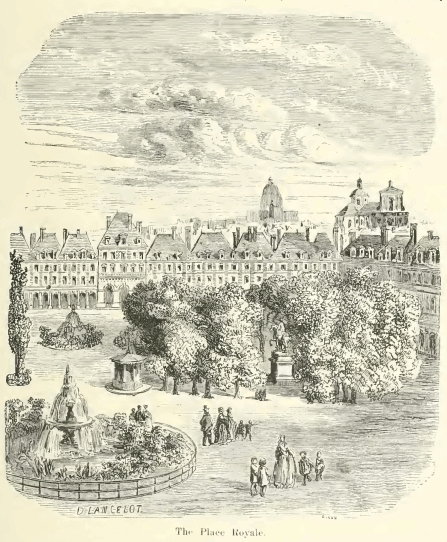
\includegraphics[width=\textwidth]{40260m.jpg}
\end{figure}

“I will remember it,” said the young man, “as selfish children
recollect their parents when they want their aid. When I need your
assistance, and the moment arrives, I will come to you, count.”

“Well, I rely upon your promise. Good-bye, then.”

“Good-bye, till we meet again.”

They had arrived in the Champs-Élysées. Monte Cristo opened the
carriage-door, Morrel sprang out on the pavement, Bertuccio was waiting
on the steps. Morrel disappeared down the Avenue de Marigny, and Monte
Cristo hastened to join Bertuccio.

“Well?” asked he.

“She is going to leave her house,” said the steward.

“And her son?”

“Florentin, his valet, thinks he is going to do the same.”

“Come this way.” Monte Cristo took Bertuccio into his study, wrote the
letter we have seen, and gave it to the steward. “Go,” said he quickly.
“But first, let Haydée be informed that I have returned.”

“Here I am,” said the young girl, who at the sound of the carriage had
run downstairs and whose face was radiant with joy at seeing the count
return safely. Bertuccio left. Every transport of a daughter finding a
father, all the delight of a mistress seeing an adored lover, were felt
by Haydée during the first moments of this meeting, which she had so
eagerly expected. Doubtless, although less evident, Monte Cristo’s joy
was not less intense. Joy to hearts which have suffered long is like
the dew on the ground after a long drought; both the heart and the
ground absorb that beneficent moisture falling on them, and nothing is
outwardly apparent.

Monte Cristo was beginning to think, what he had not for a long time
dared to believe, that there were two Mercédès in the world, and he
might yet be happy. His eye, elate with happiness, was reading eagerly
the tearful gaze of Haydée, when suddenly the door opened. The count
knit his brow.

“M. de Morcerf!” said Baptistin, as if that name sufficed for his
excuse. In fact, the count’s face brightened.

“Which,” asked he, “the viscount or the count?”

“The count.”

“Oh,” exclaimed Haydée, “is it not yet over?”

“I know not if it is finished, my beloved child,” said Monte Cristo,
taking the young girl’s hands; “but I do know you have nothing more to
fear.”

“But it is the wretched——”

“That man cannot injure me, Haydée,” said Monte Cristo; “it was his son
alone that there was cause to fear.”

“And what I have suffered,” said the young girl, “you shall never know,
my lord.”

Monte Cristo smiled. “By my father’s tomb,” said he, extending his hand
over the head of the young girl, “I swear to you, Haydée, that if any
misfortune happens, it will not be to me.”

“I believe you, my lord, as implicitly as if God had spoken to me,”
said the young girl, presenting her forehead to him. Monte Cristo
pressed on that pure beautiful forehead a kiss which made two hearts
throb at once, the one violently, the other secretly.

“Oh,” murmured the count, “shall I then be permitted to love again? Ask
M. de Morcerf into the drawing-room,” said he to Baptistin, while he
led the beautiful Greek girl to a private staircase.

We must explain this visit, which although expected by Monte Cristo, is
unexpected to our readers. While Mercédès, as we have said, was making
a similar inventory of her property to Albert’s, while she was
arranging her jewels, shutting her drawers, collecting her keys, to
leave everything in perfect order, she did not perceive a pale and
sinister face at a glass door which threw light into the passage, from
which everything could be both seen and heard. He who was thus looking,
without being heard or seen, probably heard and saw all that passed in
Madame de Morcerf’s apartments. From that glass door the pale-faced man
went to the count’s bedroom and raised with a constricted hand the
curtain of a window overlooking the courtyard. He remained there ten
minutes, motionless and dumb, listening to the beating of his own
heart. For him those ten minutes were very long. It was then Albert,
returning from his meeting with the count, perceived his father
watching for his arrival behind a curtain, and turned aside. The
count’s eye expanded; he knew Albert had insulted the count dreadfully,
and that in every country in the world such an insult would lead to a
deadly duel. Albert returned safely—then the count was revenged.

An indescribable ray of joy illumined that wretched countenance like
the last ray of the sun before it disappears behind the clouds which
bear the aspect, not of a downy couch, but of a tomb. But as we have
said, he waited in vain for his son to come to his apartment with the
account of his triumph. He easily understood why his son did not come
to see him before he went to avenge his father’s honor; but when that
was done, why did not his son come and throw himself into his arms?

It was then, when the count could not see Albert, that he sent for his
servant, who he knew was authorized not to conceal anything from him.
Ten minutes afterwards, General Morcerf was seen on the steps in a
black coat with a military collar, black pantaloons, and black gloves.
He had apparently given previous orders, for as he reached the bottom
step his carriage came from the coach-house ready for him. The valet
threw into the carriage his military cloak, in which two swords were
wrapped, and, shutting the door, he took his seat by the side of the
coachman. The coachman stooped down for his orders.

“To the Champs-Élysées,” said the general; “the Count of Monte
Cristo’s. Hurry!”

The horses bounded beneath the whip; and in five minutes they stopped
before the count’s door. M. de Morcerf opened the door himself, and as
the carriage rolled away he passed up the walk, rang, and entered the
open door with his servant.

A moment afterwards, Baptistin announced the Count of Morcerf to Monte
Cristo, and the latter, leading Haydée aside, ordered that Morcerf be
asked into the drawing-room. The general was pacing the room the third
time when, in turning, he perceived Monte Cristo at the door.

“Ah, it is M. de Morcerf,” said Monte Cristo quietly; “I thought I had
not heard aright.”

“Yes, it is I,” said the count, whom a frightful contraction of the
lips prevented from articulating freely.

“May I know the cause which procures me the pleasure of seeing M. de
Morcerf so early?”

“Had you not a meeting with my son this morning?” asked the general.

“I had,” replied the count.

“And I know my son had good reasons to wish to fight with you, and to
endeavor to kill you.”

“Yes, sir, he had very good ones; but you see that in spite of them he
has not killed me, and did not even fight.”

“Yet he considered you the cause of his father’s dishonor, the cause of
the fearful ruin which has fallen on my house.”

“It is true, sir,” said Monte Cristo with his dreadful calmness; “a
secondary cause, but not the principal.”

“Doubtless you made, then, some apology or explanation?”

“I explained nothing, and it is he who apologized to me.”

“But to what do you attribute this conduct?”

“To the conviction, probably, that there was one more guilty than I.”

“And who was that?”

“His father.”

“That may be,” said the count, turning pale; “but you know the guilty
do not like to find themselves convicted.”

“I know it, and I expected this result.”

“You expected my son would be a coward?” cried the count.

“M. Albert de Morcerf is no coward!” said Monte Cristo.

“A man who holds a sword in his hand, and sees a mortal enemy within
reach of that sword, and does not fight, is a coward! Why is he not
here that I may tell him so?”

“Sir,” replied Monte Cristo coldly, “I did not expect that you had come
here to relate to me your little family affairs. Go and tell M. Albert
that, and he may know what to answer you.”

“Oh, no, no,” said the general, smiling faintly, “I did not come for
that purpose; you are right. I came to tell you that I also look upon
you as my enemy. I came to tell you that I hate you instinctively; that
it seems as if I had always known you, and always hated you; and, in
short, since the young people of the present day will not fight, it
remains for us to do so. Do you think so, sir?”

“Certainly. And when I told you I had foreseen the result, it is the
honor of your visit I alluded to.”

“So much the better. Are you prepared?”

“Yes, sir.”

“You know that we shall fight till one of us is dead,” said the
general, whose teeth were clenched with rage.

\begin{figure}[ht]
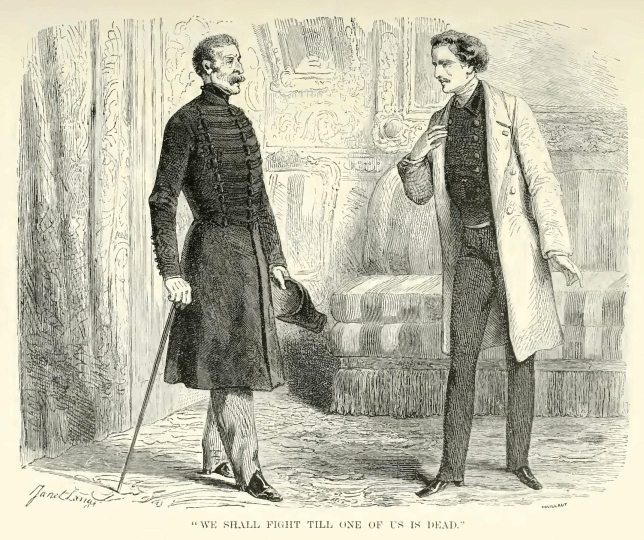
\includegraphics[width=\textwidth]{40262m.jpg}
\end{figure}

“Until one of us dies,” repeated Monte Cristo, moving his head slightly
up and down.

“Let us start, then; we need no witnesses.”

“Very true,” said Monte Cristo; “it is unnecessary, we know each other
so well!”

“On the contrary,” said the count, “we know so little of each other.”

“Indeed?” said Monte Cristo, with the same indomitable coolness; “let
us see. Are you not the soldier Fernand who deserted on the eve of the
battle of Waterloo? Are you not the Lieutenant Fernand who served as
guide and spy to the French army in Spain? Are you not the Captain
Fernand who betrayed, sold, and murdered his benefactor, Ali? And have
not all these Fernands, united, made Lieutenant-General, the Count of
Morcerf, peer of France?”

“Oh,” cried the general, as if branded with a hot iron, “wretch,—to
reproach me with my shame when about, perhaps, to kill me! No, I did
not say I was a stranger to you. I know well, demon, that you have
penetrated into the darkness of the past, and that you have read, by
the light of what torch I know not, every page of my life; but perhaps
I may be more honorable in my shame than you under your pompous
coverings. No—no, I am aware you know me; but I know you only as an
adventurer sewn up in gold and jewellery. You call yourself, in Paris,
the Count of Monte Cristo; in Italy, Sinbad the Sailor; in Malta, I
forget what. But it is your real name I want to know, in the midst of
your hundred names, that I may pronounce it when we meet to fight, at
the moment when I plunge my sword through your heart.”

The Count of Monte Cristo turned dreadfully pale; his eye seemed to
burn with a devouring fire. He leaped towards a dressing-room near his
bedroom, and in less than a moment, tearing off his cravat, his coat
and waistcoat, he put on a sailor’s jacket and hat, from beneath which
rolled his long black hair. He returned thus, formidable and
implacable, advancing with his arms crossed on his breast, towards the
general, who could not understand why he had disappeared, but who on
seeing him again, and feeling his teeth chatter and his legs sink under
him, drew back, and only stopped when he found a table to support his
clenched hand.

“Fernand,” cried he, “of my hundred names I need only tell you one, to
overwhelm you! But you guess it now, do you not?—or, rather, you
remember it? For, notwithstanding all my sorrows and my tortures, I
show you today a face which the happiness of revenge makes young
again—a face you must often have seen in your dreams since your
marriage with Mercédès, my betrothed!”

\begin{figure}[ht]
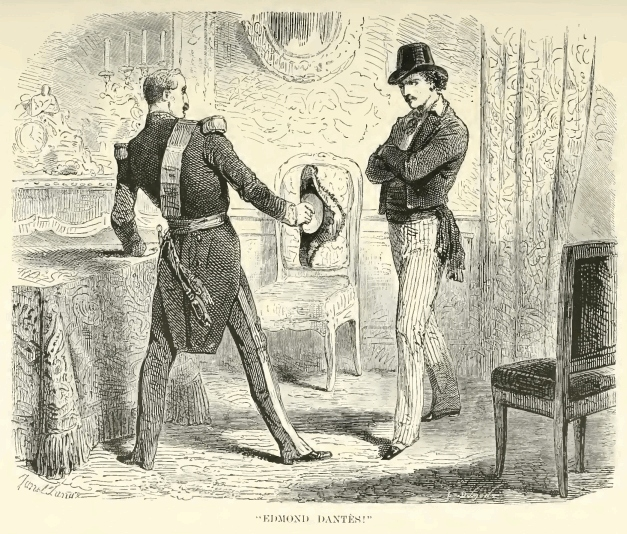
\includegraphics[width=\textwidth]{40268m.jpg}
\end{figure}

The general, with his head thrown back, hands extended, gaze fixed,
looked silently at this dreadful apparition; then seeking the wall to
support him, he glided along close to it until he reached the door,
through which he went out backwards, uttering this single mournful,
lamentable, distressing cry:

“Edmond Dantès!”

Then, with sighs which were unlike any human sound, he dragged himself
to the door, reeled across the courtyard, and falling into the arms of
his valet, he said in a voice scarcely intelligible,—“Home, home.”

The fresh air and the shame he felt at having exposed himself before
his servants, partly recalled his senses, but the ride was short, and
as he drew near his house all his wretchedness revived. He stopped at a
short distance from the house and alighted. The door was wide open, a
hackney-coach was standing in the middle of the yard—a strange sight
before so noble a mansion; the count looked at it with terror, but
without daring to inquire its meaning, he rushed towards his apartment.

Two persons were coming down the stairs; he had only time to creep into
an alcove to avoid them. It was Mercédès leaning on her son’s arm and
leaving the house. They passed close by the unhappy being, who,
concealed behind the damask curtain, almost felt Mercédès dress brush
past him, and his son’s warm breath, pronouncing these words:

“Courage, mother! Come, this is no longer our home!”

The words died away, the steps were lost in the distance. The general
drew himself up, clinging to the curtain; he uttered the most dreadful
sob which ever escaped from the bosom of a father abandoned at the same
time by his wife and son. He soon heard the clatter of the iron step of
the hackney-coach, then the coachman’s voice, and then the rolling of
the heavy vehicle shook the windows. He darted to his bedroom to see
once more all he had loved in the world; but the hackney-coach drove on
and the head of neither Mercédès nor her son appeared at the window to
take a last look at the house or the deserted father and husband.

And at the very moment when the wheels of that coach crossed the
gateway a report was heard, and a thick smoke escaped through one of
the panes of the window, which was broken by the explosion.

\begin{figure}[ht]
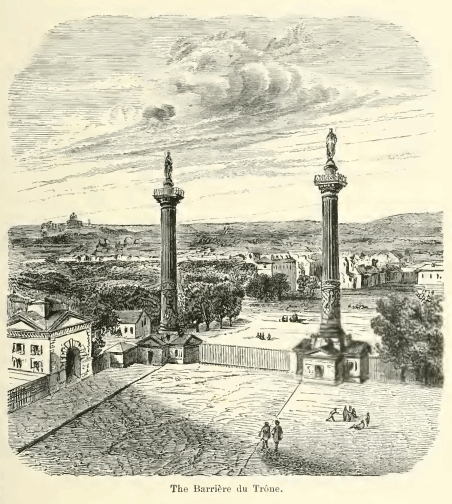
\includegraphics[width=\textwidth]{40270m.jpg}
\end{figure}
